\subsection*{The Left-Digit Effect and Stock Selling Behavior}

Investors are more likely to sell stocks after a change in the left-digit. This occurs for both price increases and decreases. The likelihood of a stock being sold jumps when the price crosses the left-digit from below, e.g. a stock increasing from \pounds9 to \pounds10, and also increases when the price crosses the left-digit from above, e.g. a stock decreasing from \pounds10 to \pounds9. We interpret this as showing that investor attention is drawn to stocks that change their leftmost digit. Left-digit changes are attention grabbing, causing sale activity. This is similar to the rank effect finding of Hartzmark (2015), whereby either top-ranked or bottom-ranked stocks by return since purchase are those most likely to be sold.

To show our result, we draw a sample of stock $\times$ quarters that have increased in value and have gone through a left-digit in a calendar quarter (e.g. Jan - Mar), which we call the Price Increasing Sample. We then draw a sample of stocks that have decreased in value through a left-digit in a calendar quarter, which we call the Price Decreasing Sample.\footnote{We have implemented this sample restriction approximately in this version. In a future version we will implement the sample restriction precisely. We do not expect the results to change when we do this.} Note, this sample restriction is at the stock $\times$ quarter level.

We then draw all investor $\times$ stock $\times$ days within the Price Increasing Sample and the Price Decreasing Sample, i.e. all observations for investors $\times$ days on which the investor held the stock at the beginning of the day. We look at the probability of sale when the stock is just below a left-digit change, e.g. \pounds9, compared with above the left-digit change, e.g. \pounds10. This exercise might compare investor $\times$ stock $\times$ days drawn from different investors. Therefore, we also conduct estimates that include individual fixed effects, thereby exploiting within-investor variation in the probability of sale either side of the left-digit change.

\ref{fig:left_digit_sell} illustrates the main result. Each panel shows the probability of a stock sale by the leftmost two digits of the stock price. Note, this pools over leftmost digits that are in pence, pounds, hundreds of pounds, and so on. The only information used in the analysis is the leftmost two digits, in integer values. The left-side plots pool all observations by the leftmost two digits and the probability of sale together with a 95\% confidence interval. The right-side plots show the probability of sale by leftmost two digits. Panel A shows an increase in the probability of sale when the price crosses the left-digit from below, Panel B shows an increase in the probability of sale when the price crosses the left-digit from above. \ref{fig:left_digit_sell_increase} and \ref{fig:left_digit_sell_decrease} reproduce these plots for subsamples by the price range of the stock, in Panel A up to \pounds1, in Panel B between \pounds1 and \pounds10, and in Panel C between \pounds10 and \pounds100.

Possible queries:
\begin{itemize}
	\item [1] Limit orders. We have previously discussed the possibility that the patterns we see might be created by limit orders set at left-digit thresholds, i.e., round numbers. We think this is not the general mechanism at work, because limit orders would create a spike in the probability of sale at the left-digit alone. It would not explain the increased probability of sale at X1, X2, etc.. We think we see higher probability at X1, X2, etc.. because there is a delay between the stock crossing the left-digit and investors logging-in to their accounts. We could examine the role of limit orders more precisely by looking into very fine price data at the penny level.
	\item [2] Sample selection. We have previously discussed the possibility that the results might in some way be an artefact of sample selection, given that we are selecting on stock $\times$ quarters that pass through a left digit change. We can clarify any concerns around sample selection in two ways. 
	\begin{itemize}
		\item [A] It is true that our sample selection criteria mean that our sample does not uniformly comprise observations across XO - X9. For example, in the price increasing sample the requirement is that the stock has increased in value up to at least X0, but there is no further requirement. This will give us an excess of observations at X0 compared with X1, X2, and so on. We see this is indeed the case in \ref{fig:sample_selection_test} in the histogram. However, this does not bias our results as the y-variable in our analysis is the \textit{probability} of sale. Hence, the XO bin has a larger denominator in the y-variable compared with the other variables. Moreover, our results is that the probability of sales increases between X9 and X0, for which there is only a small increase in density in the histogram.
		\item [B] To double-check, we conducted a simulation analysis in which we input the same data but choose stocks to be sold at random. The result in \ref{fig:sample_selection_test} in the right-side plot confirms that this delivers a uniform probability of sale. 
	\end{itemize}
\end{itemize}

\clearpage

\begin{figure}[hbt!]
	\caption{Leftmost Stock Price Digit and Probability of Sale}%
	\label{fig:left_digit_sell}%
	\centering%	
	\bigskip
	\subfigure[Price Increasing]{
			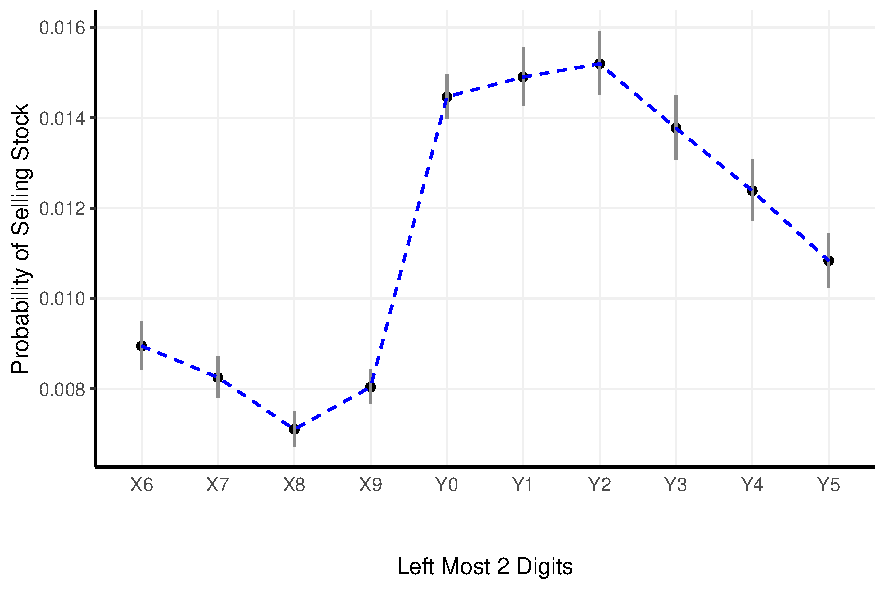
\includegraphics[width=0.45\textwidth]{figures/Left2increase_probCI.pdf}
			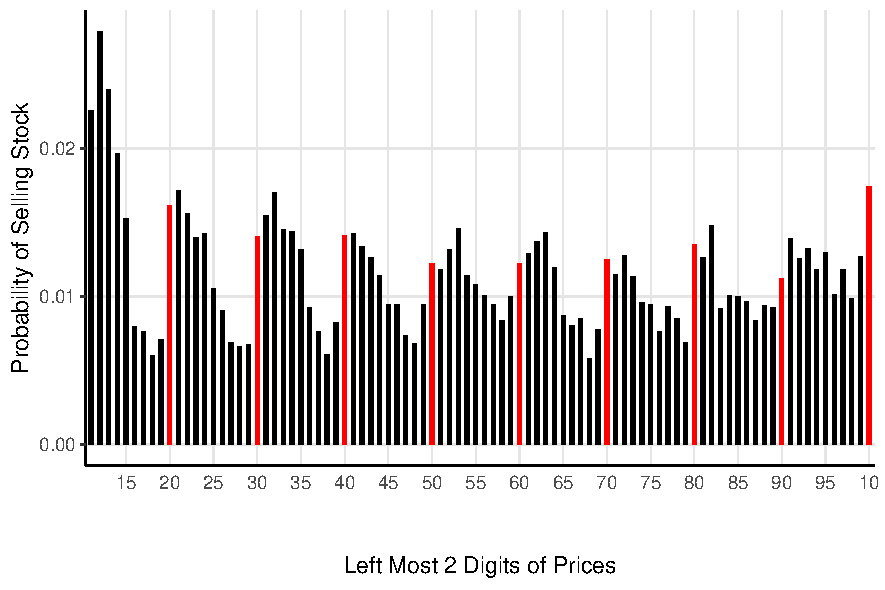
\includegraphics[width=0.45\textwidth]{figures/2left_increase.pdf}	
	}
	\subfigure[Price Decreasing]{
		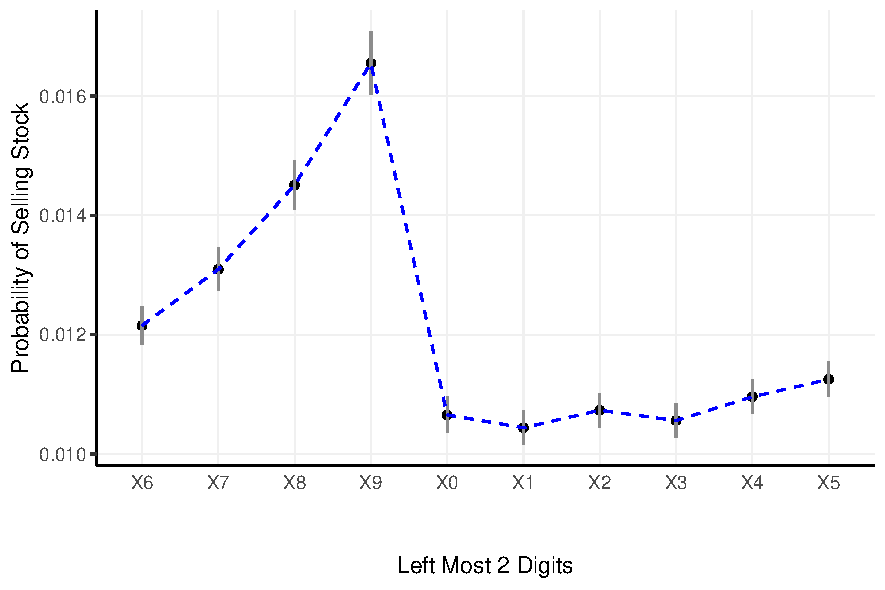
\includegraphics[width=0.45\textwidth]{figures/Left2decrease_probCI.pdf}
		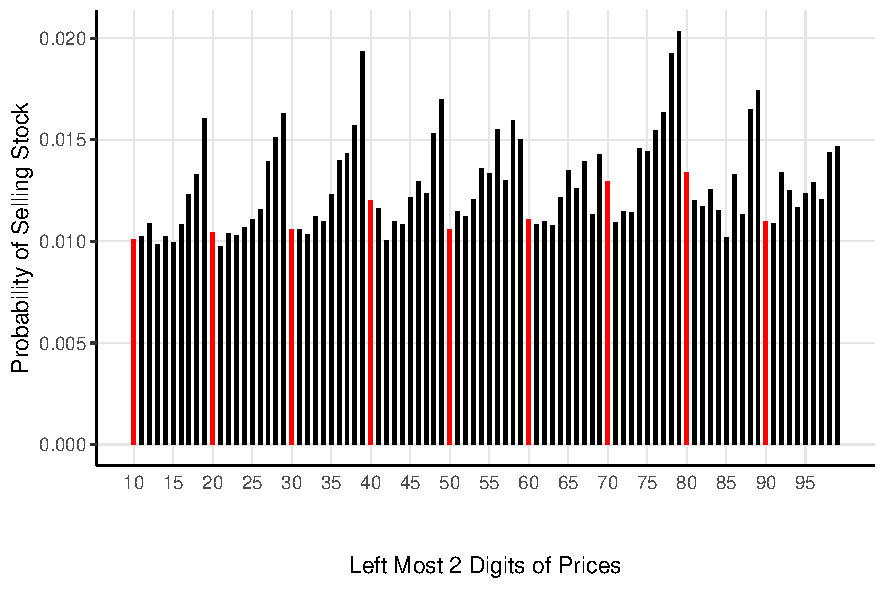
\includegraphics[width=0.45\textwidth]{figures/2left_decrease.pdf}	
	}
\end{figure}

\clearpage

\begin{figure}[hbt!]
	\caption{Leftmost Stock Price Digit and Probability of Sale \\ Prices Increasing Sample by Price Range}%
	\label{fig:left_digit_sell_increase}%
	\centering%	
	\bigskip
		\subfigure[Price = \pounds0.11 to \pounds1.01]{
			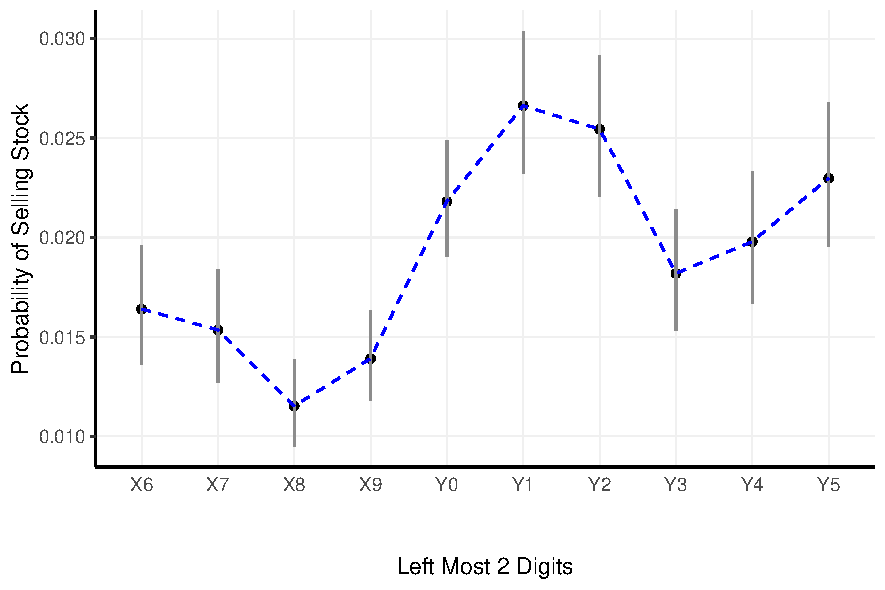
\includegraphics[width=0.45\textwidth]{figures/Left2increases_1pbin_CI.pdf}
			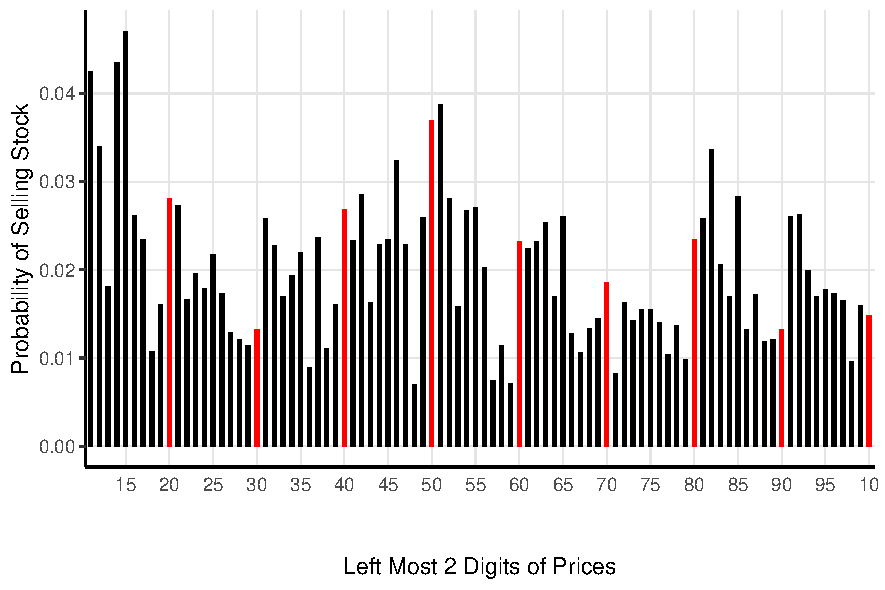
\includegraphics[width=0.45\textwidth]{figures/2left_increase_bin1p.pdf}
		}
		\subfigure[Price = \pounds1.01 to \pounds10.1]{
			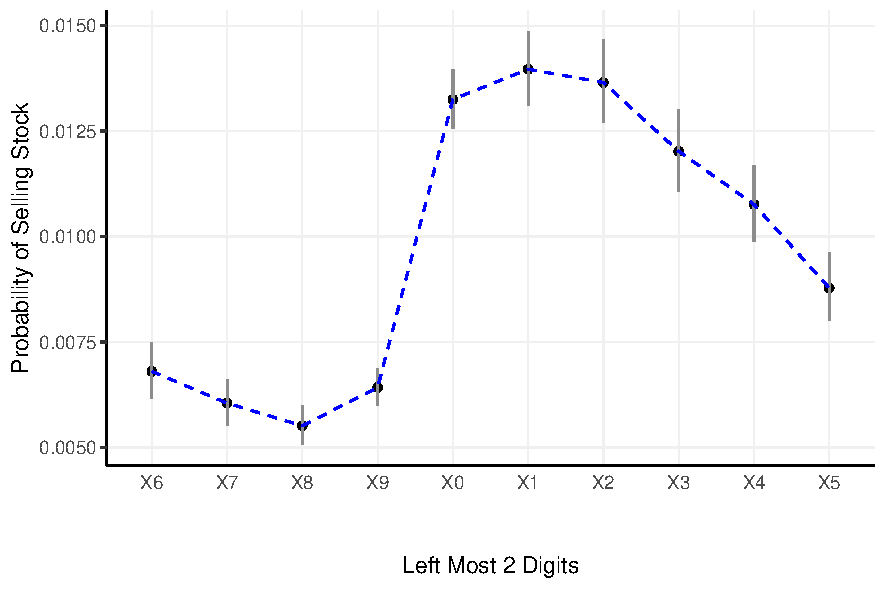
\includegraphics[width=0.45\textwidth]{figures/Left2increases_10pbin_CI.pdf}
			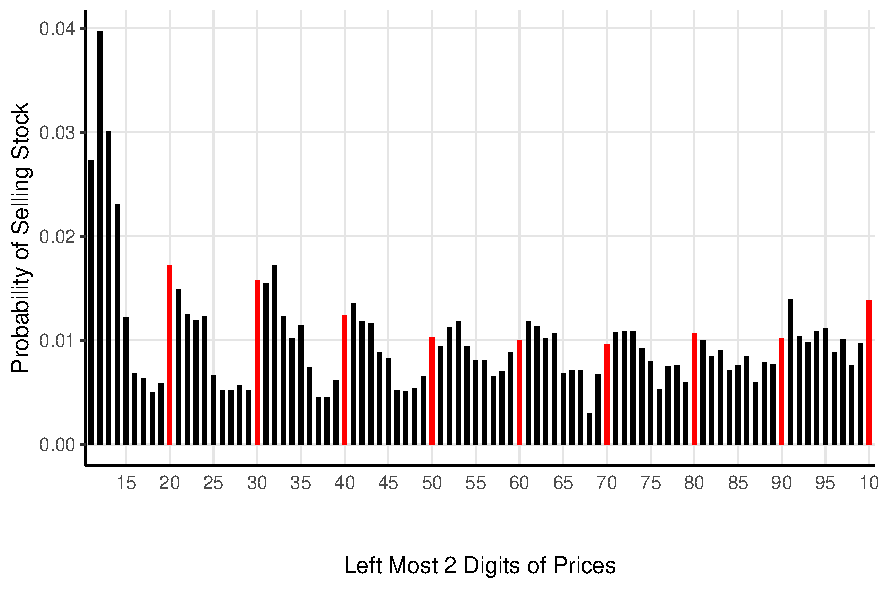
\includegraphics[width=0.45\textwidth]{figures/2left_increase_bin10p.pdf}
		}
		\subfigure[Price = \pounds11 to \pounds101]{
			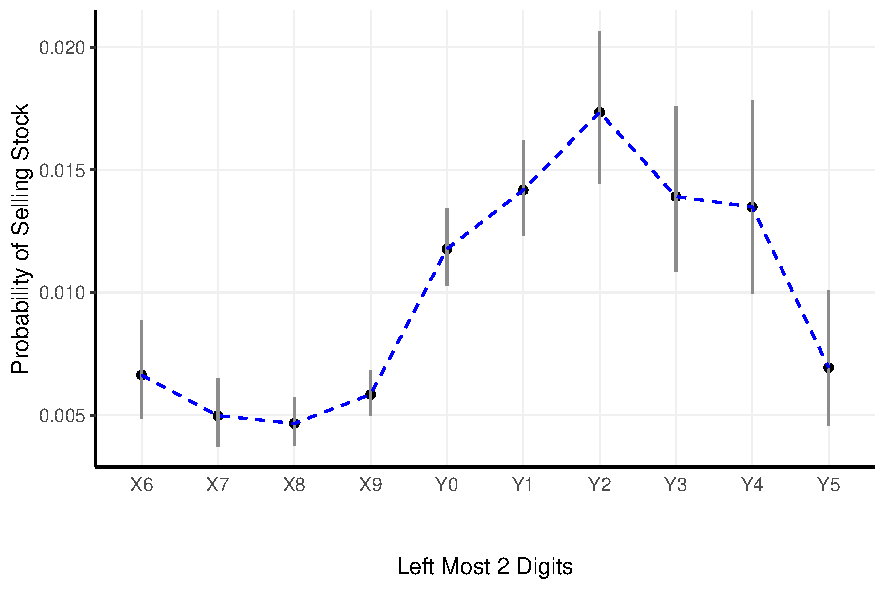
\includegraphics[width=0.45\textwidth]{figures/Left2increases_1poundbin_CI.pdf}
			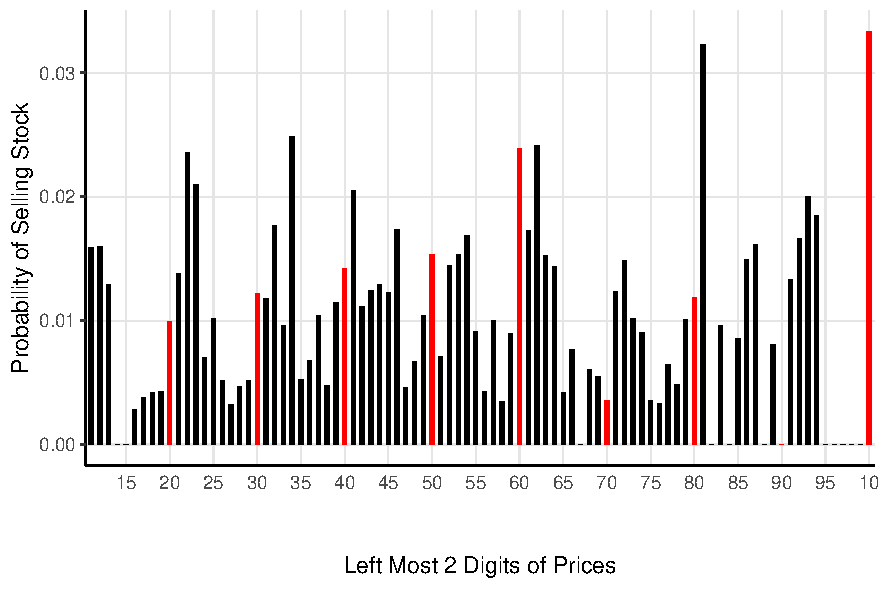
\includegraphics[width=0.45\textwidth]{figures/2left_increase_bin1pound.pdf}
		}
\end{figure}

\begin{figure}[hbt!]
	\caption{Leftmost Stock Price Digit and Probability of Sale \\ Prices Decreasing Sample by Price Range}%
	\label{fig:left_digit_sell_decrease}%
	\centering%	
	\bigskip
	\subfigure[Price = \pounds0.11 to \pounds1.01]{
		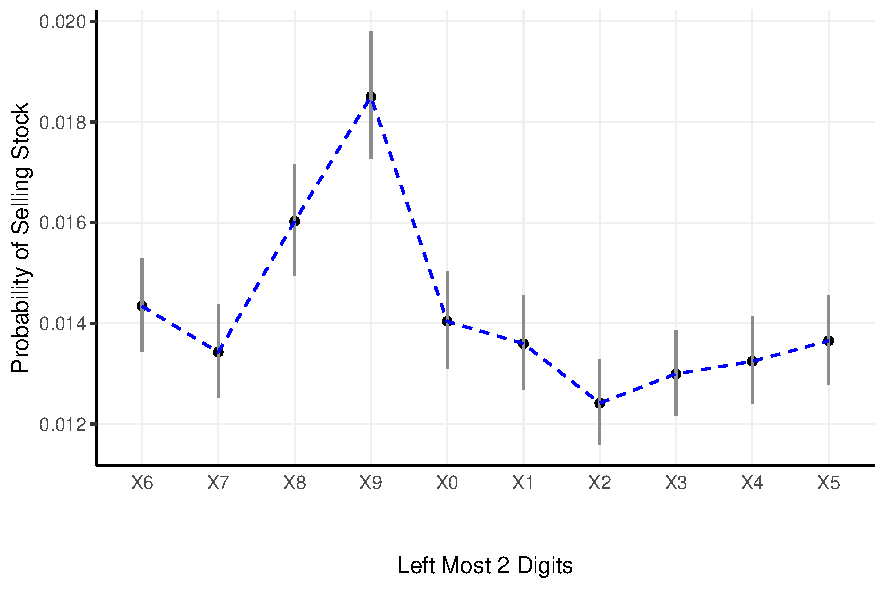
\includegraphics[width=0.45\textwidth]{figures/Left2decreases_1pbin_CI.pdf}
		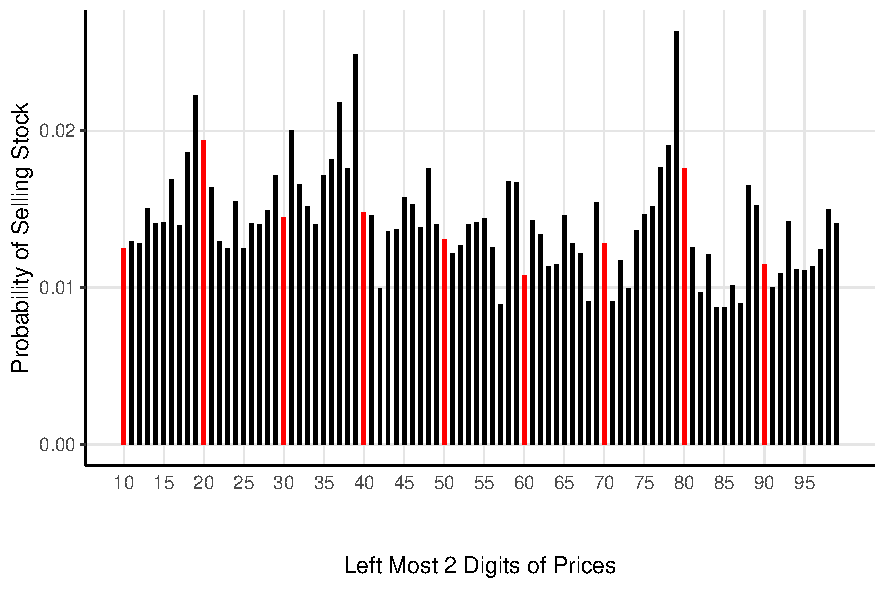
\includegraphics[width=0.45\textwidth]{figures/2left_decrease_bin1p.pdf}
	}
	\subfigure[Price = \pounds1.01 to \pounds10.1]{
		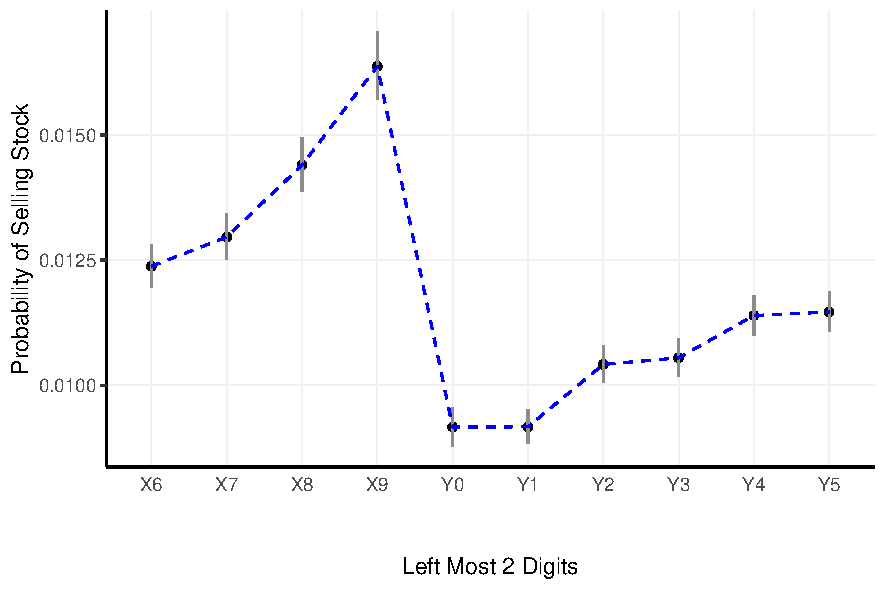
\includegraphics[width=0.45\textwidth]{figures/Left2decreases_10pbin_CI.pdf}
		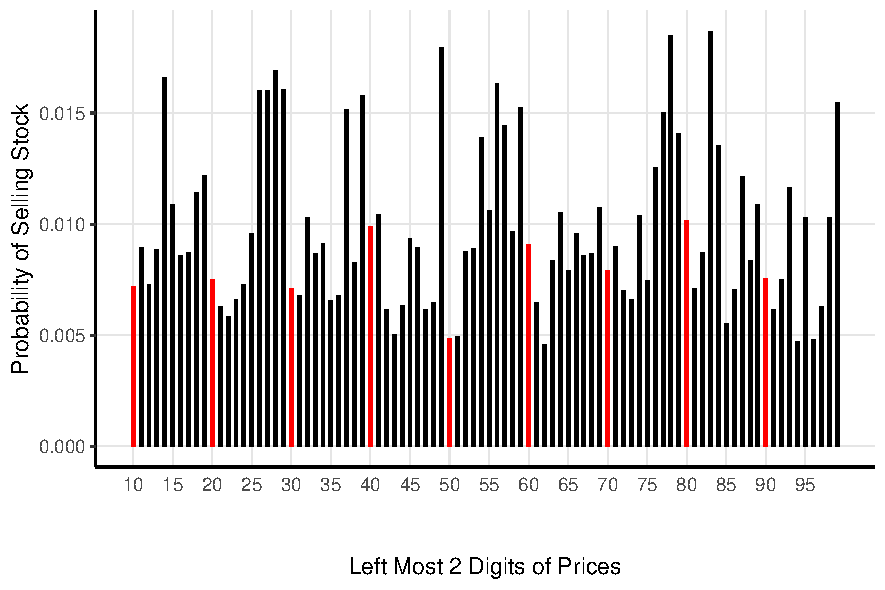
\includegraphics[width=0.45\textwidth]{figures/2left_decrease_bin10p.pdf}
	}
	\subfigure[Price = \pounds11 to \pounds101]{
		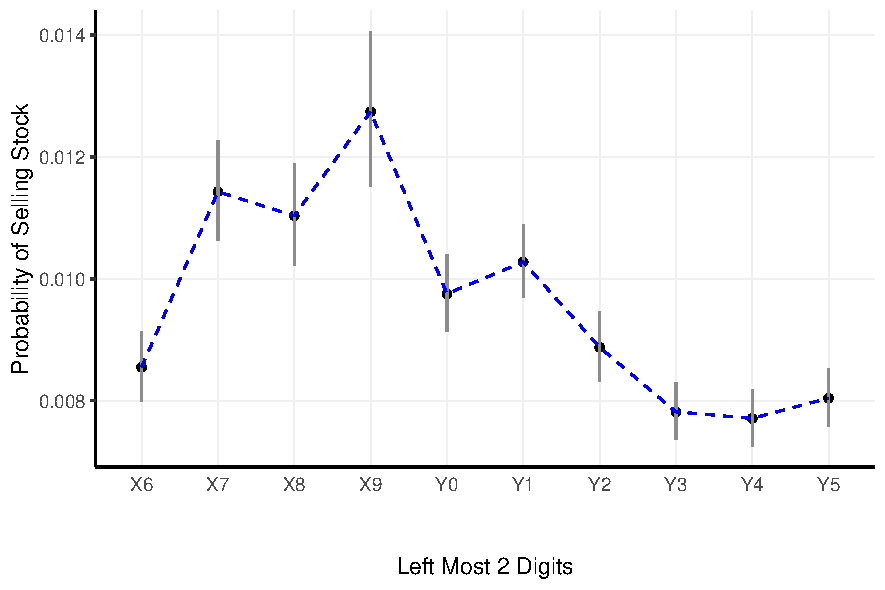
\includegraphics[width=0.45\textwidth]{figures/Left2decreases_1poundbin_CI.pdf}
		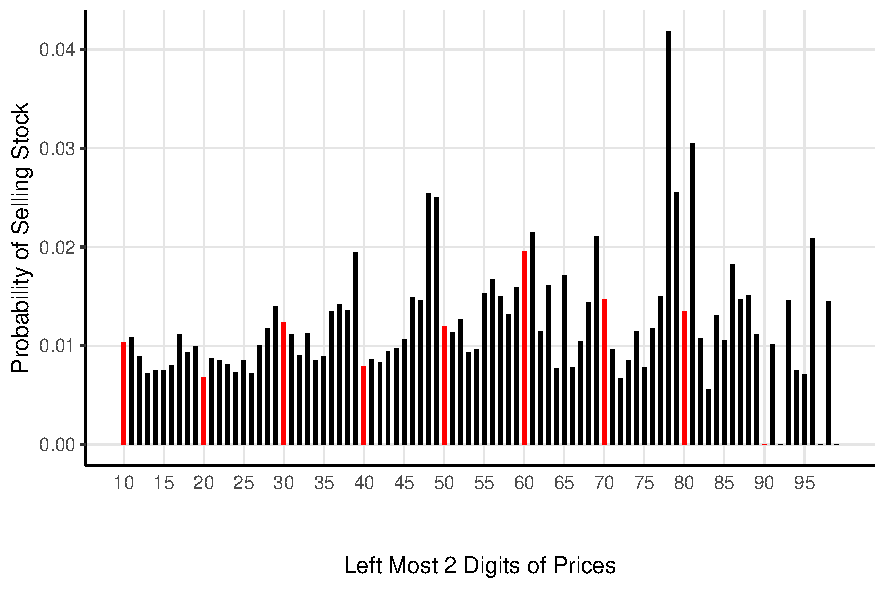
\includegraphics[width=0.45\textwidth]{figures/2left_decrease_bin1pound.pdf}
	}
\end{figure}

\clearpage

\begin{econtable}[h]\footnotesize
	\caption{Probability of Sale and Left Digit, Price Increasing Sample}
	\label{tab:regressions_increase}
	\estauto{l c c c c c c  }{
		& \multicolumn{5}{c}{$Probability\:  of\:  Sale_{ijt}=1$} \\ 
		%	\cmidrule(rr){2-7}
		& \multicolumn{1}{c}{(1)} & \multicolumn{1}{c}{(2)} & \multicolumn{1}{c}{(3)} & \multicolumn{1}{c}{(4)} & 
		\multicolumn{1}{c}{(5)} & \\ 
		\midrule
		\\[-2.1ex] Above X0 = 1 & 0.0058{***} & 0.0076{***} & 0.0070{***} & 0.0067{***} & 0.0070{***} \\ 
  & (0.0002) & (0.0003) & (0.0003) & (0.0003) & (0.0003) \\ 
  Stock Digits (XO to X5) &  & -0.0007{***} & -0.0008{***} & -0.0008{***} & -0.0010{***} \\ 
  &  & (0.0001) & (0.0001) & (0.0001) & (0.0001) \\ 
  Stock Digits (X6 to X9) &  & -0.0003{***} & -0.0001 & -0.0001 & 0.0001 \\ 
  &  & (0.0001) & (0.0001) & (0.0001) & (0.0001) \\ 
  Constant & 0.0080{***} & 0.0076{***} & 0.0098{***} &  &  \\ 
  & (0.0003) & (0.0003) & (0.0025) &  &  \\ 
 Day FE & NO & NO & YES & YES & YES \\ 
Industry FE & NO & NO & YES & YES & YES \\ 
Account FE & NO & NO & NO & YES & YES \\ 
Stock FE & NO & NO & NO & NO & YES \\ 
Observations & \multicolumn{1}{c}{1,517,823} & \multicolumn{1}{c}{1,517,823} & \multicolumn{1}{c}{1,517,823} & \multicolumn{1}{c}{1,517,823} & \multicolumn{1}{c}{1,517,823} \\ 
R$^{2}$ & \multicolumn{1}{c}{0.0008} & \multicolumn{1}{c}{0.0008} & \multicolumn{1}{c}{0.0022} & \multicolumn{1}{c}{0.0511} & \multicolumn{1}{c}{0.0549} \\ 
 
	}
	\fignote{The unit of observation is an investor $\times$ stock $\times$ day. The samples is restricted to login days. We include only quarters in which the stocks increased in price (regarding the first observation of the quarter) and change the left most digit at least once during the quarter. Only those stocks that have changed the left most digit are included. Regressions fit an intercept for the change in the left most digit at X0 and two slopes for the left (X6 to X9) and right (X0 to X5) values, as described by the raw patterns in \ref{fig:prob_all_inc}. The constant shows the probability to sell the stock at when the second digit is 9 (X9). The second digit over threshold dummy shows the jump in probability when the first digit changes and so the second digit becomes 0 (X0). SE are clustered by account.}
\end{econtable}

\clearpage

\begin{econtable}[h]\footnotesize
	\caption{Probability of Sale and Left Digit, Price Decreasing Sample}
	\label{tab:regressions_decrease}
	\estauto{l c c c c c c  }{
		& \multicolumn{5}{c}{$Probability\:  of\:  Sale_{ijt}=1$} \\ 
		%	\cmidrule(rr){2-7}
		& \multicolumn{1}{c}{(1)} & \multicolumn{1}{c}{(2)} & \multicolumn{1}{c}{(3)} & \multicolumn{1}{c}{(4)} & 
		\multicolumn{1}{c}{(5)} & \\ 
		\midrule
		\\[-2.1ex] Second Digit Over Threshold = 1 (in Range X0 to X5) & -0.0029{***} & -0.0057{***} & -0.0056{***} & -0.0054{***} & -0.0057{***} \\ 
  & (0.0001) & (0.0003) & (0.0003) & (0.0003) & (0.0003) \\ 
  Second Digit Over Threshold (= 0 to 5, corresponding to X0 to X5) &  & 0.0001{***} & 0.0002{***} & 0.0004{***} & 0.0004{***} \\ 
  &  & (0.0000) & (0.0000) & (0.0000) & (0.0000) \\ 
  Second Digit Below Threshold (= -3 to 0, corresponding to X6 to X9) &  & 0.0014{***} & 0.0013{***} & 0.0011{***} & 0.0011{***} \\ 
  &  & (0.0001) & (0.0001) & (0.0001) & (0.0001) \\ 
  Constant & 0.0137{***} & 0.0162{***} & 0.0193{***} &  &  \\ 
  & (0.0003) & (0.0004) & (0.0019) &  &  \\ 
 Day FE & NO & NO & YES & YES & YES \\ 
Industry FE & NO & NO & YES & YES & YES \\ 
Account FE & NO & NO & NO & YES & YES \\ 
Stock FE & NO & NO & NO & NO & YES \\ 
Observations & \multicolumn{1}{c}{4,376,352} & \multicolumn{1}{c}{4,376,352} & \multicolumn{1}{c}{4,376,352} & \multicolumn{1}{c}{4,376,352} & \multicolumn{1}{c}{4,376,352} \\ 
R$^{2}$ & \multicolumn{1}{c}{0.0002} & \multicolumn{1}{c}{0.0002} & \multicolumn{1}{c}{0.0009} & \multicolumn{1}{c}{0.0492} & \multicolumn{1}{c}{0.0526} \\ 
 
	}
	\fignote{The unit of observation is an investor $\times$ stock $\times$ day. The samples is restricted to login days. We include only quarters in which the stocks have not increased in price (regarding the first observation of the quarter) and have not changed the left most digit at least once during the quarter. Regressions fit an intercept for the change in the left most digit at X0 and two slopes for the left (X6 to X9) and right (X0 to X5) values, as described by the raw patterns in \ref{fig:prob_all_dec}. The constant shows the probability to sell the stock at when the second digit is 9 (X9). The second digit over threshold dummy shows the jump in probability when the first digit changes and so the second digit becomes 0 (X0). SE are clustered by account.}
\end{econtable}

\clearpage

\appendix

\begin{figure}%
	\centering%
	\caption{Histogram of Stock Prices}%
	\label{fig:histogram_prices}%
	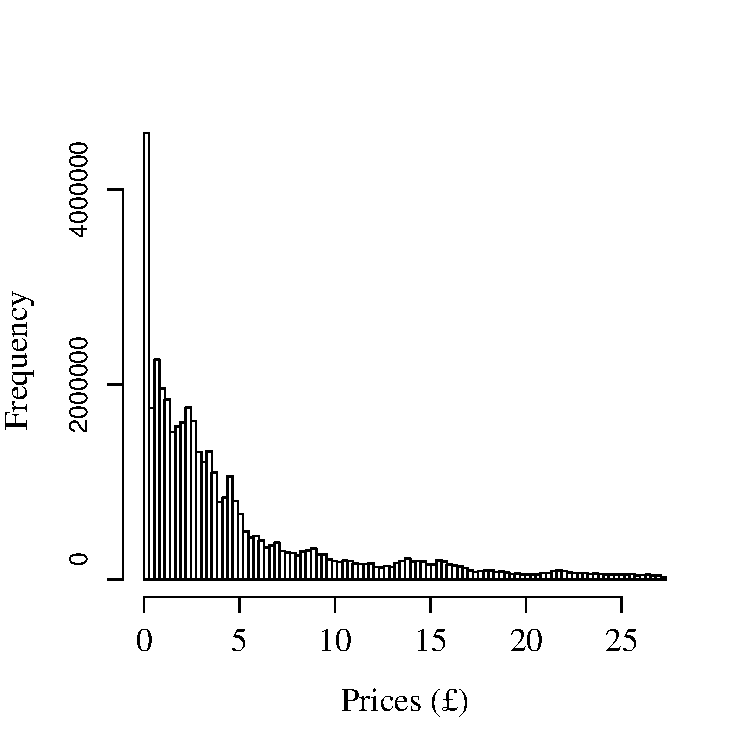
\includegraphics[width=.6\textwidth]{figures/prices_hist_login_days.pdf}
	\fignote{Figure shows the histogram of prices on login days. Outliers in the 99 percentile are excluded.}
\end{figure}

\clearpage

\begin{figure}[hbt!]
	\caption{Sample Selection and Simulation Exercise}%
	\label{fig:sample_selection_test}%
	\centering%	
	\bigskip
	\subfigure[Price Increasing Sample]{
		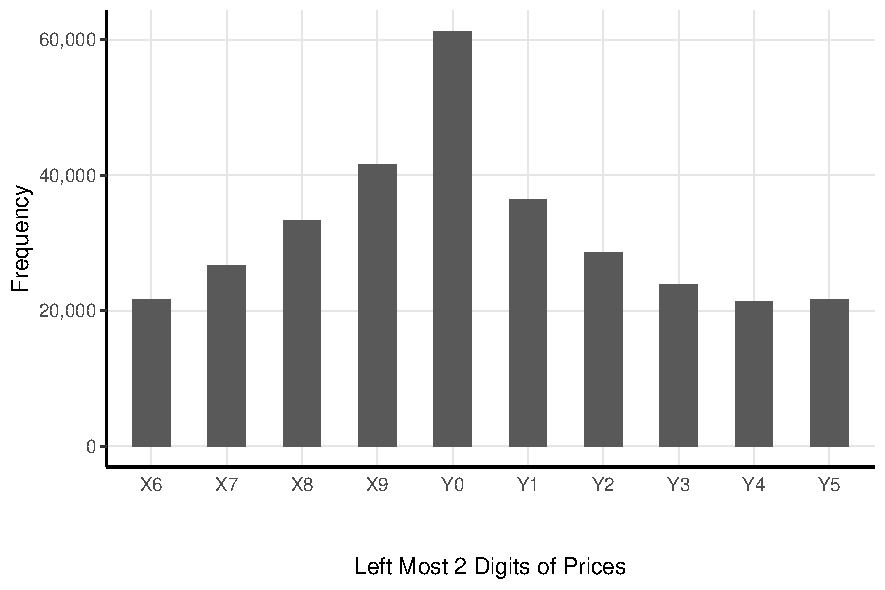
\includegraphics[width=0.45\textwidth]{figures/left2_second_increase_count.pdf}
		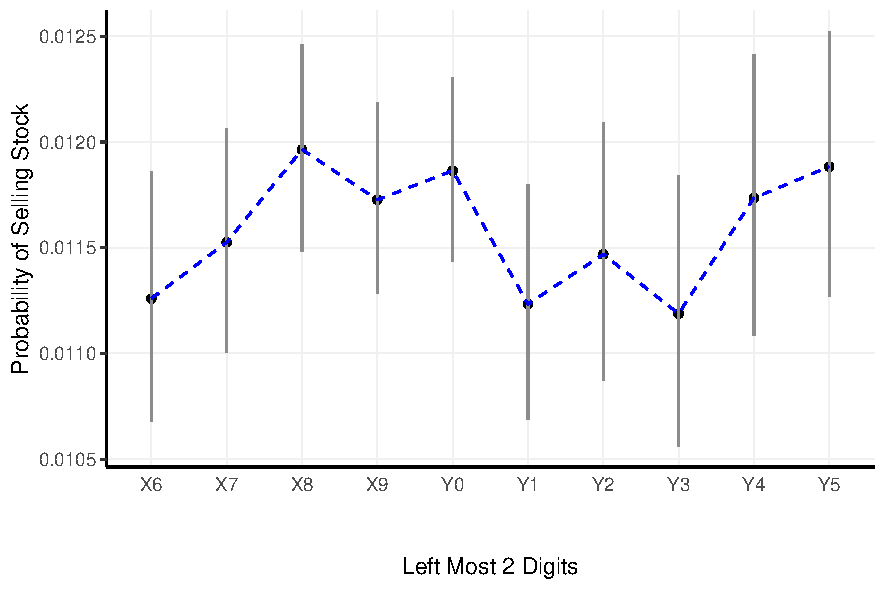
\includegraphics[width=0.45\textwidth]{figures/Left2increase_probCI_random_sell.pdf}
	}
\end{figure}


\begin{figure}%
	\centering%
	\caption{Probability of Buying}%
	\label{fig:histogram_prices}%
	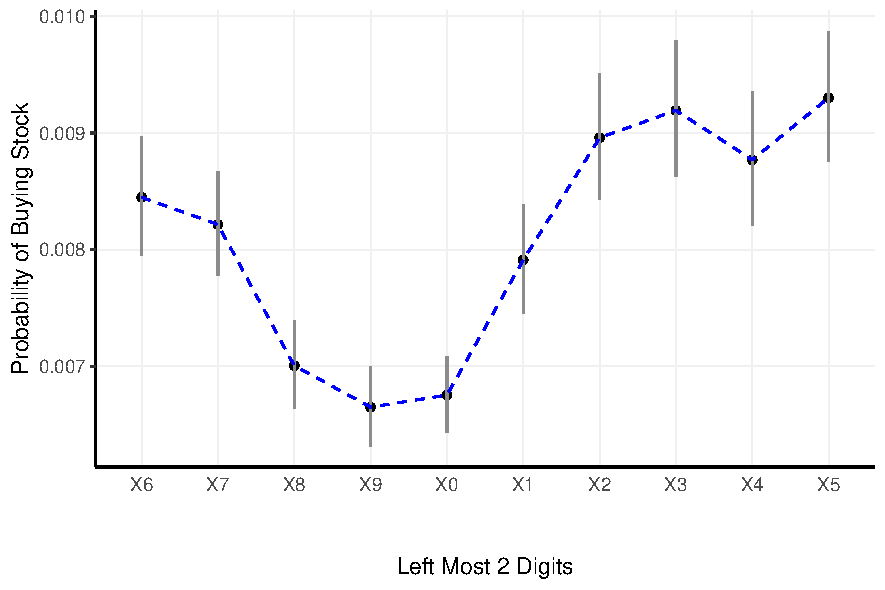
\includegraphics[width=.6\textwidth]{figures/Left2increase_probCI_buy.pdf}
	\fignote{Figure shows the probability of buying an stock under the same sample selection.}
\end{figure}

\clearpage

\begin{table}\small
	\caption{Summary Stats}
	\label{tab:price_summary_stats}
	\bigskip
	\begin{adjustbox}{center}
		\estauto{lcccccccccc}<\multicolumn{9}{c}{Panel (A): Baseline Sample} \\>{
		& \multicolumn{1}{c}{N} & \multicolumn{1}{c}{Mean} & \multicolumn{1}{c}{St. Dev.} & \multicolumn{1}{c}{Min} & \multicolumn{1}{c}{Pctl(25)} & \multicolumn{1}{c}{Median} & \multicolumn{1}{c}{Pctl(75)} & \multicolumn{1}{c}{Max} \\ 	
		Price on Login Days \pounds & 43,903,112 & 7.942 & 26.178 & 0.000 & 1.153 & 3.050 & 7.642 & 15,051.630 \\ 
Price on Sell Days \pounds & 3,341,054 & 7.103 & 24.523 & 0.000 & 0.832 & 2.646 & 6.674 & 3,589.000 \\ 
Price of Stocks Sold \pounds & 342,277 & 6.848 & 16.483 & 0.000 & 0.861 & 2.714 & 6.648 & 1,771.425 \\ 
 
	}
	\end{adjustbox}
	
	\bigskip
		
	\begin{adjustbox}{center}
		\estauto{lcccccccccc}<\multicolumn{9}{c}{Panel (B): Price Increasing Sample} \\>{
			& \multicolumn{1}{c}{N} & \multicolumn{1}{c}{Mean} & \multicolumn{1}{c}{St. Dev.} & \multicolumn{1}{c}{Min} & \multicolumn{1}{c}{Pctl(25)} & \multicolumn{1}{c}{Median} & \multicolumn{1}{c}{Pctl(75)} & \multicolumn{1}{c}{Max} \\ 	
			All Stocks & 316,242 & 5.777 & 15.384 & 0.000 & 0.582 & 2.433 & 6.010 & 2,001.557 \\ 
Stocks with Prices Between \pounds 0.11 to \pounds 1.01 & 82,932 & 0.588 & 0.254 & 0.110 & 0.378 & 0.616 & 0.795 & 1.010 \\ 
Stocks with Prices Between \pounds 1.1 to \pounds 10.1 & 155,842 & 4.816 & 2.367 & 1.100 & 2.917 & 4.348 & 6.578 & 10.099 \\ 
Stocks with Prices Between \pounds 11 to \pounds 101 & 25,401 & 34.166 & 18.423 & 11.000 & 19.931 & 30.040 & 46.290 & 100.690 \\ 
 
		}
	\end{adjustbox}
	
	\bigskip
		
	\begin{adjustbox}{center}
		\estauto{lcccccccccc}<\multicolumn{9}{c}{Panel (C): Price Decreasing Sample} \\>{
			& \multicolumn{1}{c}{N} & \multicolumn{1}{c}{Mean} & \multicolumn{1}{c}{St. Dev.} & \multicolumn{1}{c}{Min} & \multicolumn{1}{c}{Pctl(25)} & \multicolumn{1}{c}{Median} & \multicolumn{1}{c}{Pctl(75)} & \multicolumn{1}{c}{Max} \\ 	
			All Stocks & 4,376,352 & 7.507 & 26.412 & 0.000 & 1.183 & 2.650 & 8.270 & 4,495.251 \\ 
Stocks with Prices Between \pounds 0.10 to \pounds 1.0 & 611,813 & 0.491 & 0.277 & 0.100 & 0.226 & 0.472 & 0.740 & 1.000 \\ 
Stocks with Prices Between \pounds 1 to \pounds 10 & 2,461,228 & 3.230 & 1.998 & 1.000 & 1.750 & 2.602 & 4.176 & 10.000 \\ 
Stocks with Prices Between \pounds 10 to \pounds 100 & 978,415 & 20.993 & 11.905 & 10.000 & 13.725 & 16.350 & 24.450 & 99.990 \\ 
 
		}
	\end{adjustbox}
\end{table}

